\chapter{Modelos de Redes Neurais}
\label{ch:03}


% \epigraph{\itshape Those who cannot remember the past are condemned to compute it.''}{---Steven Pinker, \textit{Words and Rules}}

Este Capítulo serve como uma introdução à teoria das redes neurais. Os conceitos introduzidos neste Capítulo servirão como embasamento teórico imprescindível para a apresentação do modelo final utilizado nesta pesquisa, o \textit{Encoder-Decoder}. 

\section{Introdução a Redes Neurais}

Um modelo de rede neural é, essencialmente, um modelo de aprendizado de máquina supervisionado %[ref] 
que está a procura de identificar padrões. Um modelo de aprendizado de máquina é uma tarefa computacional que explora algoritmos que podem aprender a partir de seus erros e fazer previsões sobre dados. Esse tipo de algoritmo é normalmente inicializado com nenhuma expectativa sobre a tarefa que deve realizar e busca informações exclusivamente a partir dos dados do problema. Os possíveis tipos de aprendizado de máquina são divididos entre: \textit{supervisionados}, \textit{não-supervisionados}
e por \textit{reforço}. (ref)
No caso das redes neurais, o aprendizado diz-se supervisionado, pois informa-se ao modelo o \textit{output} esperado  pelo treinamento (o \textit{alvo}) para cada informação de entrada (cada \textit{input}).

A inspiração para o desenvolvimento da modelagem em redes neurais aritificiais surgiu a partir de estudos em neurosciência %[ref] 
que concluiram que, diante de múltiplas apresentações de um mesmo estímulo, um mesmo conjunto de neurônios sofre incitação e dispara. Um estímulo diferente resulta no disparo de um conjunto de neurônios diferente (\cite{hubel:1962}).  Analogamente, o modelo artificial é composto por uma camada denominada de \textit{input} responsável por receber diferentes estímulos (matematicamente retratados por vetores numéricos que representam o objeto do aprendizado). A informação recebida é distribuída ao longo de múltiplas conexões com a próxima camada através de uma multiplicação com uma matriz de pesos $\vect{W}$. A matriz de pesos funciona como uma analogia às conexões existentes entre neurônios de modo que um peso maior representa uma conexão reforçada e um peso menor representa uma conexão reprimida. Além disso, é importante que o sistema de aprendizado não seja demasiado sensível a todo \textit{input} que receber, pois nesse caso cada \textit{input} diferente recebido alteraria completamente o modelo impossibilitando um aprendizado generalizado. Como solução, o resultado obtido a partir da multiplicação dos pesos pelos \textit{inputs} entra como argumento em uma função, que nesse contexto é chamada de \textit{função de ativação}. A função de ativação é uma função que simula o potencial energético existente entre as conexões neurais e permite que uma unidade apenas seja ativada caso o resultado dessa função atinja um limiar mínimo. Isso permite ao sistema a produção de diferentes respostas para padrões diferentes utilizando a mesma rede e além disso, permite que o aprendizado ocorra de forma gradual, de modo que o efeito de estímulos passados ainda perdure por um longo período mesmo após a apresentação de novos estímulos. Uma das funções de ativação mais utilizadas na literatura (e inclusive utilizada pelos pesquisadores Rumelhart e McClelland) é a função \textit{Sigmoid}, uma função suave, diferenciável e facilmente interpretável. A Fig. \ref{fig:sigmoidplot} ilustra o processo de ativação dado um \textit{input} $\vect{x}$. Supõe-se que um neurônio seja ativado apenas se houver uma energia mínima para tal. Da mesma forma, representa-se uma ativação no eixo \textit{y} (com valores entre 0 (não ativação) e 1 (ativação)) de modo que apenas valores mais altos de $\vect{x}$ atingem valores próximos da ativação em \textit{y}.

\begin{figure}[H]
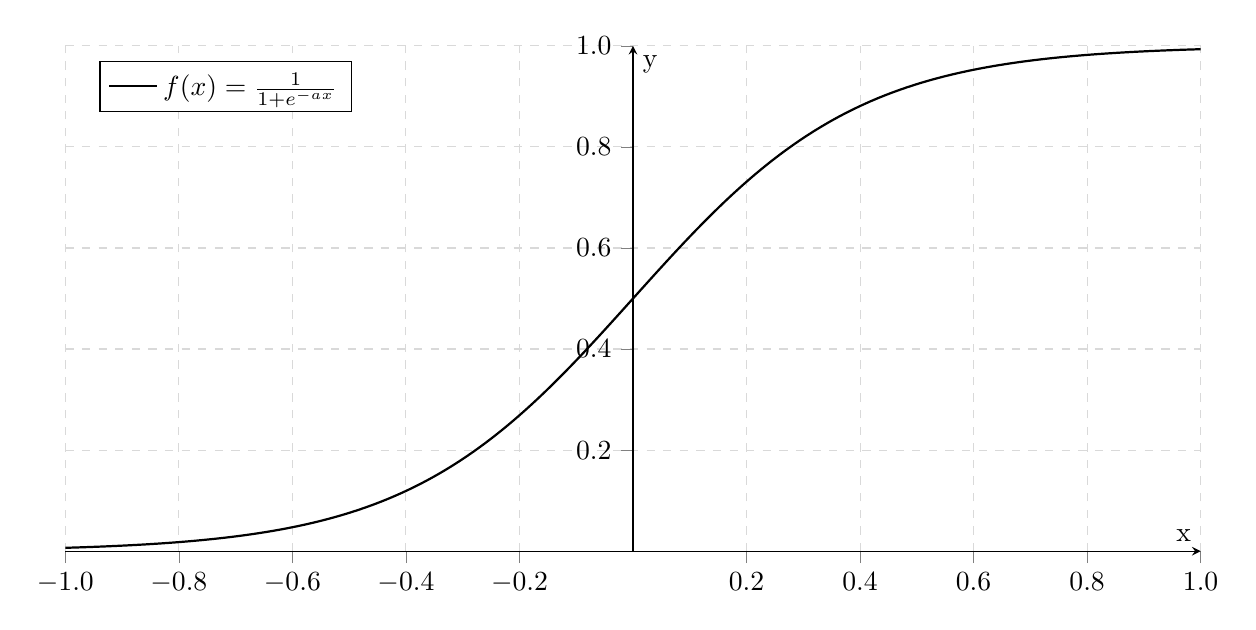
\begin{tikzpicture}
    \begin{axis}[
    	legend pos=north west,
        axis x line=middle,
        axis y line=middle,
        x tick label style={/pgf/number format/fixed,
                            /pgf/number format/fixed zerofill,
                            /pgf/number format/precision=1},
        y tick label style={/pgf/number format/fixed,
                            /pgf/number format/fixed zerofill,
                            /pgf/number format/precision=1},
        grid = major,
        width=16cm,
        height=8cm,
        grid style={dashed, gray!30},
        xmin=-1,     % start the diagram at this x-coordinate
        xmax= 1,    % end   the diagram at this x-coordinate
        ymin= 0,     % start the diagram at this y-coordinate
        ymax= 1,   % end   the diagram at this y-coordinate
        %axis background/.style={fill=white},
        xlabel=x,
        ylabel=y,
        tick align=outside,
        enlargelimits=false]
      % plot the stirling-formulae
      \addplot[domain=-1:1, black, thick,samples=500] {1/(1+exp(-5*x))};
      %\addplot[domain=-1:1, blue, ultra thick,samples=500] {1/(1+exp(-10*x))};
      \addlegendentry{$f(x)=\frac{1}{1+e^{-ax}}$}
      %\addlegendentry{$g(x)=\frac{1}{1+e^{-10x}}$}
    \end{axis} 
\end{tikzpicture}
\caption{A função logística utilizada para o cálculo da probabilidade de ativação.}
\label{fig:sigmoidplot}
\end{figure} %diminuir esse desenho

Após essa passagem pela função de ativação, o resultado serve como novo input para a próxima camada e assim sucessivamente até a última, a camada de \textit{output}. Todas as camadas existentes entre as camadas de \textit{input} e de \textit{output} são chamadas de \textit{camadas escondidas} (Ver Fig. \ref{fig:ffd}.)

% \begin{align}\label{eq:sigmoid}
% p(w_{i} = 1) = \frac{1}{1+e^{\sum_{i} w_{i}x_{i}}}
% \end{align}

Algebricamente, pode-se representar o processo descrito através da composição de múltiplas funções, uma vez que o resultado das operações precedentes servirão como entrada para as próximas camadas.

\begin{align}
% f(\vect{x}) &= f^{(2)}(f^{(1)}(\vect{x}; \vect{W}_1); \vect{W}_2)\\
% &= 
\sigma(\vect{W}_2 (\sigma(\vect{W}_1\vect{x})))
\end{align}

\definecolor{blue}{RGB}{159, 192, 176}
\definecolor{green}{RGB}{160, 227, 127}
\definecolor{orange}{RGB}{243, 188, 125}
\definecolor{red}{RGB}{253, 123, 84}
\definecolor{nephritis}{RGB}{39, 174, 96}
\definecolor{emerald}{RGB}{46, 204, 113}
\definecolor{turquoise}{RGB}{39, 174, 96}
\definecolor{green-sea}{RGB}{22, 160, 133}
\definecolor{purple}{RGB}{181, 124, 215}
% Tikzstyles for Computation Graphs

% nodes
\tikzstyle{noop} = [circle, draw=none, fill=red, minimum size = 10pt]
\tikzstyle{op} = [circle, draw=red, line width=1.5pt, fill=red!70, text=black, text centered, font=\bf \normalsize, minimum size = 25pt]

\tikzstyle{opintense} = [circle, draw=red, line width=1.5pt, fill=red!150, text=black, text centered, font=\bf \normalsize, minimum size = 25pt]


%new style
\tikzstyle{gp} = [circle, draw=red, line width=4pt, text=black, text centered, font=\bf \normalsize, minimum size = 4.cm]

\tikzstyle{box} = [rectangle, draw=red, line width=1.5pt, fill=red!70, text=black, align=center, font=\bf \normalsize, minimum size = 45pt]

\tikzstyle{box2} = [rectangle, draw=black, line width=0.9pt, text=black, align=center, font=\bf \normalsize, minimum size = 20pt]

\tikzstyle{box3} = [rectangle, draw=black, line width=0.9pt, fill=black, text=black, align=center, font=\bf \normalsize, minimum size = 20pt]

\tikzstyle{state} = [circle, draw=blue, line width=1.5pt, fill=blue!70, text=black, text centered, font=\bf \normalsize, minimum size = 25pt]

\tikzstyle{output} = [circle, draw=purple, line width=1.5pt, fill=purple!70, text=black, text centered, font=\bf \normalsize, minimum size = 25pt]


\tikzstyle{gradient} = [circle, draw=nephritis, line width=1.5pt, fill=nephritis!60, text=black, text centered, font=\bf \normalsize, minimum size = 25pt]
\tikzstyle{textonly} = [draw=none, fill=none, text centered, font=\bf \normalsize]
\tikzstyle{boxtextonly} = [draw=none, fill=none, align=center, font=\bf \normalsize]

\tikzstyle{normal} = [circle, draw=black, line width=1.0pt, fill=none, text=black, text centered, font=\bf \normalsize, minimum size = 20pt]


% edges
\tikzstyle{tedge}  = [draw, thick, >=latex, ->]
\tikzstyle{tedge_dashed}  = [draw, thick, >=latex, ->, dashed]
\tikzstyle{nedge}  = [draw, thick, >=latex]
\tikzstyle{nedge_dashed}  = [draw, thick, >=latex, dashed]


% namedscope
\tikzstyle{namedscope} = [circle, draw=orange, line width=1.5pt, fill=orange!60, align=center, inner sep=0pt]
\begin{figure}[ht!]
\centering

\scalebox{1.0}{
\begin{tikzpicture}[auto]

% operations =========

% FNN input
\node[normal] (x1) {};
\node[textonly, above=10pt of x1] (input) {Camada de \textit{inputs}};
\node[normal, below=10pt of x1] (x2) {};
\node[normal, below=10pt of x2] (x3) {};
\node[normal, below=10pt of x3] (x4) {};
\node[normal, below=10pt of x4] (x5) {};
\node[normal, below=10pt of x5] (x6) {};

% FNN output
\node[textonly, right=50pt of x1] (center) {Camada Escondida};
\node[normal, below=25pt of center] (y1) {};
\node[normal, below=10pt of y1] (y2) {};
\node[normal, below=10pt of y2] (y3) {};

% FNN output
\node[textonly, right=110pt of input] (output) {Camada de \textit{outputs}};
\node[normal, below=15pt of output] (z1) {};

\node[normal, below=10pt of z1] (z2) {};
\node[normal, below=10pt of z2] (z3) {};
\node[normal, below=10pt of z3] (z4) {};
\node[normal, below=10pt of z4] (z5) {};
\node[normal, below=10pt of z5] (z6) {};

% phon features 2

% edges FNN
\path[nedge] (x1) -- (y1);
\path[nedge] (x1) -- (y2);
\path[nedge] (x1) -- (y3);

\path[nedge] (x2) -- (y1);
\path[nedge] (x2) -- (y2);
\path[nedge] (x2) -- (y3);

\path[nedge] (x3) -- (y1);
\path[nedge] (x3) -- (y2);
\path[nedge] (x3) -- (y3);

\path[nedge] (x4) -- (y1);
\path[nedge] (x4) -- (y2);
\path[nedge] (x4) -- (y3);

\path[nedge] (x5) -- (y1);
\path[nedge] (x5) -- (y2);
\path[nedge] (x5) -- (y3);

\path[nedge] (x6) -- (y1);
\path[nedge] (x6) -- (y2);
\path[nedge] (x6) -- (y3);

% edges FNN
\path[nedge] (y1) -- (z1);
\path[nedge] (y1) -- (z2);
\path[nedge] (y1) -- (z3);
\path[nedge] (y1) -- (z4);
\path[nedge] (y1) -- (z5);
\path[nedge] (y1) -- (z6);
\path[nedge] (y2) -- (z1);
\path[nedge] (y2) -- (z2);
\path[nedge] (y2) -- (z3);
\path[nedge] (y2) -- (z4);
\path[nedge] (y2) -- (z5);
\path[nedge] (y2) -- (z6);
\path[nedge] (y3) -- (z1);
\path[nedge] (y3) -- (z2);
\path[nedge] (y3) -- (z3);
\path[nedge] (y3) -- (z4);
\path[nedge] (y3) -- (z5);
\path[nedge] (y3) -- (z6);

\end{tikzpicture}
}\caption{Esquema de uma rede neural do tipo Feedforward} 
\label{fig:ffd}
\end{figure}

\subsection{Treinamento}

Para que a rede seja capaz de identificar os padrões desejados, é necessário alimentá-la também com o que se espera como resposta (\textit{targets} ou \textit{alvos}), pois o treinamento da mesma consiste, essencialmente, na atualização das matrizes de pesos que deve ocorrer a partir da comparação entre os valores previstos pela rede (os \textit{outputs}) e os \textit{targets}. A comparação entre esses valores se dá por meio de uma função de custo (\textit{Loss Function}), que representa uma forma de se quantificar o quão perto se está de uma rede ideal em que os resultados previstos correspondam exatamente aos \textit{targets}. O objetivo do aprendizado da rede é minimizar essa diferença, ou seja, encontrar os valores dos pesos na matriz $\vect{W}$ que minimizam a função de custo (\cite{josh:2017}). Para isso, faz-se uso de um algoritmo chamado de \textit{backpropagation} (ref). Após a inserção de cada input e a aplicação do algoritmo de backpropagation, todos os pesos de $\vect{W}$ são atualizados simultaneamente com os valores que em conjunto minimizam a função de custo e portanto aproximam as previsões da rede aos alvos. Entretanto, o ajuste de um modelo de redes neurais é bastante delicado e experimental. Ele depende não somente da busca pelos melhores parâmetros de $\vect{W}$ como também de uma busca pelos chamados \textit{hiperparâmetros}. 

Os hiperparâmetros são parâmetros do modelo que são escolhidos a priori para configurar o modelo. Um deles refere-se ao número de vezes em que um mesmo input é inserido no modelo, conhecido como o número de \textit{épocas}. Existem também outros hiperparâmetros importantes como a taxa de aprendizado $\eta$, o parâmetro de regularização $\lambda$, dimensões de camadas escondidas, número de camadas escondidas, entre outros (ref). Todos esses hiperparâmetros definem as configurações do treinamento e juntos podem levar ao sucesso ou insucesso do aprendizado. A escolha dos melhores hiperparâmetros para um modelo de redes neurais não é tarefa trivial. Múltiplos treinamentos com diferentes configurações de hiperparâmetros são realizados para que se possa fazer essa escolha. Na prática, porém, é mais comum que esses hiperparâmetros sejam configurados a partir de resultados de experimentos semelhantes publicados na literatura.   

Mesmo com uma extensa busca pelos hiperparâmetros do modelo, nem sempre é possível encontrar valores em $\vect{W}$ que possibilitem o aprendizado de forma satisfatória. Na prática, é bastante comum a ocorrência de problemas conhecidos como \textit{overfit} (quando o modelo se torna especialista nos dados de treino mas tem dificuldade de generalizar para dados nunca vistos antes) e \textit{underfit} (quando o modelo falha em capturar o padrão subjacente dos dados) (ref). Na literatura existem algumas técnicas disponíveis para tratar dessas questões, como Dropout, Data Augmentation e Over ou Under Sampling (ref). Ainda assim, o modelo de redes neurais é um modelo cuja interpretabilidade mostra-se ainda bastante inacessível, o que torna o resultado do treinamento bastante hermético. (ref)   %ref 

\section{Uma Outra Arquitetura}
\label{sec:arqFDD}
%juntar o cap 4 aqui dentro
O esquema apresentado pelos pesquisadores Rumelhart e McClelland represetado na Fig. \ref{fig:esquemafdd} é conhecido como uma arquitetura do tipo \textit{Feedforward-Network (FFD)} sem camadas escondidas. Nesse caso, todos os nódulos da camada de input se conectam diretamente aos nódulos da camada de output.

Com esse modelo foi possível atingir uma acurácia de x\% na tarefa de aprendizado de verbos do Simple Past da língua inglesa. Entretanto a arquitetura do tipo FFD não é a mais adequada para dados sequenciais. No Cap. \ref{ch:02} foi abordado o complicado esquema de codificação dos verbos através de trigramas de traços distintivos. O processo de decodificação dos mesmos era ainda mais complicado e envolvia um esquema de competição entre trigramas, ver referencia tal tal tal. \cite{Pinker:1999} inclusive comenta sobre a dificuldade de decodificação da palavra 'algalgal' (uma palavra da língua Oykangand). Como a representação do output da rede FFD aponta apenas a presença ou ausência dos traços, e não quantas vezes eles aparecem, o processo de decodificação apresenta problemas e a rede dificilmente acerta em casos de verbos maiores ou com repetições de trigramas de traços. No caso da língua portuguesa, essa tarefa é bastante difícil pois os verbos são em média maiores que os verbos da língua inglesa (como comentado no \ref{ch:01}). 

Com isso, introduz-se um novo tipo de rede conhecida como Rede Neural Recorrente (RNN) cuja arquitetura foi pensada para esse caso de dados sequenciais. Para entender o funcionamento desse tipo de rede, antes faz-se necessária uma introdução ao conceito de \textit{Modelo de Linguagem}.

\subsection{Modelo de Linguagem}

Um modelo de linguagem é um modelo que propõe uma distribuição probabilística para uma sequência de termos em uma linguagem natural. Em outras palavras, um modelo de linguagem responde à pergunta: "dados os termos $x_1,x_2,x_3,x_4$, qual a probabilidade deles ocorrerem em uma determinada sequência?"

A forma clássica de se abordar esse problema se dá através da assunção de independência entre os termos da sequência em combinação à Regra do Produto de Probabilidades, ou seja, considera-se que a probabilidade de uma determinada sequência com $T$ termos acontecer é igual à probabilidade da $palavra_{t}$ ocorrer dado que as outras $t-1$ palavras ocorreram:

\begin{equation}
P(x_1, \dots, x_T) = \prod_{t=1}^{T} P(x_t \vert x_1, \dots, x_{t-1}) 
\end{equation}

Essas considerações deram origem aos modelos de $N$-Gramas. Diferentes valores para N dão origem a diferentes modelos. O modelo de unigrama, por exemplo, leva em consideração apenas a probabilidade de cada termo da sequência:

\begin{equation}
P_{uni}(x_1, x_2, x_3, x_4) = P(x_1)P(x_2)P(x_3)P(x_4)
\end{equation}

Em que $P(x_i) = contagem(x_i)$ e $contagem$ é uma função que conta a ocorrência dessa palavra no corpus.\\

A partir de N=2, ou seja, do modelo de \textit{bigramas}, esse tipo de modelagem começa a fazer mais sentido. A ideia é calcular a probabilidade dos termos dada a contagem de vezes em que eles ocorreram um após o outro em um corpus de treinamento.

\begin{equation}
P_{bi}(x_1,x_2,x_3,x_4) = P(x_1)P(x_2\vert x_1)P(x_3\vert x_2)P(x_4\vert x_3)
\end{equation} 
em que
\begin{equation}
P(x_i\vert x_j) = \frac{contagem(x_i, x_j)}{contagem(x_j)}

Esse tipo de modelo de linguagem, apesar de intuitivo, apresenta alguns obstáculos. O primeiro deles é o fato de atribuir probabilidade 0 se uma sequência de termos específica não existe no corpus de treinamento. Outro grande problema é o número alto de computações das probabilidades conforme o texto aumenta de tamanho ou o \textit{N} do \textit{N-Grama} aumenta. Desse modo fica difícil de se manter uma coerência dentro de uma sentença, o que se vê na prática são frases constituídas de "remendos", pequenos grupos de (\textit{N}) palavras que produzem uma janela muito pequena de sentido.

\subsection{Redes Neurais Recorrentes}
\label{sec:RNN}

Os modelos de Redes Neurais Recorrentes (ref) surgem como uma alternativa ao tradicional modelo de linguagem de \textit{N-Gramas}. A ideia central desse modelo consiste na retroalimentação dos elementos sequenciais, de modo que o \textit{input} de cada um deles serve, não somente para a previsão do próximo item da sequência, mas também para a formação de um componente intermediário, um \textit{estado}. Esses estados, representados na Figura \ref{fig:unfoldedrnn} como $\vect{h}$'s são matrizes que funcionam como uma espécie de memória condensada dos elementos precedentes e servem como input para os estados posteriores. Essa é uma maneira de retransmitir a cada momento os efeitos dos \textit{inputs} anteriores para o restante da sequência (\cite{Goodfellow-et-al-2016}). 

%\definecolor{blue}{RGB}{159, 192, 176}
\definecolor{green}{RGB}{160, 227, 127}
\definecolor{orange}{RGB}{243, 188, 125}
\definecolor{red}{RGB}{253, 123, 84}
\definecolor{nephritis}{RGB}{39, 174, 96}
\definecolor{emerald}{RGB}{46, 204, 113}
\definecolor{turquoise}{RGB}{39, 174, 96}
\definecolor{green-sea}{RGB}{22, 160, 133}
\definecolor{purple}{RGB}{181, 124, 215}
% Tikzstyles for Computation Graphs

% nodes
\tikzstyle{noop} = [circle, draw=none, fill=red, minimum size = 10pt]
\tikzstyle{op} = [circle, draw=red, line width=1.5pt, fill=red!70, text=black, text centered, font=\bf \normalsize, minimum size = 25pt]

\tikzstyle{opintense} = [circle, draw=red, line width=1.5pt, fill=red!150, text=black, text centered, font=\bf \normalsize, minimum size = 25pt]


%new style
\tikzstyle{gp} = [circle, draw=red, line width=4pt, text=black, text centered, font=\bf \normalsize, minimum size = 4.cm]

\tikzstyle{box} = [rectangle, draw=red, line width=1.5pt, fill=red!70, text=black, align=center, font=\bf \normalsize, minimum size = 45pt]

\tikzstyle{box2} = [rectangle, draw=black, line width=0.9pt, text=black, align=center, font=\bf \normalsize, minimum size = 20pt]

\tikzstyle{box3} = [rectangle, draw=black, line width=0.9pt, fill=black, text=black, align=center, font=\bf \normalsize, minimum size = 20pt]

\tikzstyle{state} = [circle, draw=blue, line width=1.5pt, fill=blue!70, text=black, text centered, font=\bf \normalsize, minimum size = 25pt]

\tikzstyle{output} = [circle, draw=purple, line width=1.5pt, fill=purple!70, text=black, text centered, font=\bf \normalsize, minimum size = 25pt]


\tikzstyle{gradient} = [circle, draw=nephritis, line width=1.5pt, fill=nephritis!60, text=black, text centered, font=\bf \normalsize, minimum size = 25pt]
\tikzstyle{textonly} = [draw=none, fill=none, text centered, font=\bf \normalsize]
\tikzstyle{boxtextonly} = [draw=none, fill=none, align=center, font=\bf \normalsize]

\tikzstyle{normal} = [circle, draw=black, line width=1.0pt, fill=none, text=black, text centered, font=\bf \normalsize, minimum size = 20pt]


% edges
\tikzstyle{tedge}  = [draw, thick, >=latex, ->]
\tikzstyle{tedge_dashed}  = [draw, thick, >=latex, ->, dashed]
\tikzstyle{nedge}  = [draw, thick, >=latex]
\tikzstyle{nedge_dashed}  = [draw, thick, >=latex, dashed]


% namedscope
\tikzstyle{namedscope} = [circle, draw=orange, line width=1.5pt, fill=orange!60, align=center, inner sep=0pt]
\begin{figure}[ht!]
\centering
\scalebox{1.40}{
\begin{tikzpicture}[auto]

% RNN state cell =============================
\node[normal] (h) {$\vect{h}$};
\node[normal, below=30pt of h] (x) {$\vect{x}$};
\node[normal, above=30pt of h] (yhat) {$\hat{\vect{y}}$};



% edges
\path[tedge] (x) edge node[below right= -4pt] {}  (h) ;
\path[tedge] (h) edge [out=-400,in=-320,looseness=8, distance=125pt] node[above right] {} (h);
\path[tedge] (h) edge node[below right = -4pt] {} (yhat);


\end{tikzpicture}

} % scalebox
\caption{Grafo Computacional de uma Rede Neural Recorrente}
\label{fig:rnn-cell}
\end{figure}
\definecolor{blue}{RGB}{159, 192, 176}
\definecolor{green}{RGB}{160, 227, 127}
\definecolor{orange}{RGB}{243, 188, 125}
\definecolor{red}{RGB}{253, 123, 84}
\definecolor{nephritis}{RGB}{39, 174, 96}
\definecolor{emerald}{RGB}{46, 204, 113}
\definecolor{turquoise}{RGB}{39, 174, 96}
\definecolor{green-sea}{RGB}{22, 160, 133}
\definecolor{purple}{RGB}{181, 124, 215}
% Tikzstyles for Computation Graphs

% nodes
\tikzstyle{noop} = [circle, draw=none, fill=red, minimum size = 10pt]
\tikzstyle{op} = [circle, draw=red, line width=1.5pt, fill=red!70, text=black, text centered, font=\bf \normalsize, minimum size = 25pt]

\tikzstyle{opintense} = [circle, draw=red, line width=1.5pt, fill=red!150, text=black, text centered, font=\bf \normalsize, minimum size = 25pt]


%new style
\tikzstyle{gp} = [circle, draw=red, line width=4pt, text=black, text centered, font=\bf \normalsize, minimum size = 4.cm]

\tikzstyle{box} = [rectangle, draw=red, line width=1.5pt, fill=red!70, text=black, align=center, font=\bf \normalsize, minimum size = 45pt]

\tikzstyle{box2} = [rectangle, draw=black, line width=0.9pt, text=black, align=center, font=\bf \normalsize, minimum size = 20pt]

\tikzstyle{box3} = [rectangle, draw=black, line width=0.9pt, fill=black, text=black, align=center, font=\bf \normalsize, minimum size = 20pt]

\tikzstyle{state} = [circle, draw=blue, line width=1.5pt, fill=blue!70, text=black, text centered, font=\bf \normalsize, minimum size = 25pt]

\tikzstyle{output} = [circle, draw=purple, line width=1.5pt, fill=purple!70, text=black, text centered, font=\bf \normalsize, minimum size = 25pt]


\tikzstyle{gradient} = [circle, draw=nephritis, line width=1.5pt, fill=nephritis!60, text=black, text centered, font=\bf \normalsize, minimum size = 25pt]
\tikzstyle{textonly} = [draw=none, fill=none, text centered, font=\bf \normalsize]
\tikzstyle{boxtextonly} = [draw=none, fill=none, align=center, font=\bf \normalsize]

\tikzstyle{normal} = [circle, draw=black, line width=1.0pt, fill=none, text=black, text centered, font=\bf \normalsize, minimum size = 20pt]


% edges
\tikzstyle{tedge}  = [draw, thick, >=latex, ->]
\tikzstyle{tedge_dashed}  = [draw, thick, >=latex, ->, dashed]
\tikzstyle{nedge}  = [draw, thick, >=latex]
\tikzstyle{nedge_dashed}  = [draw, thick, >=latex, dashed]


% namedscope
\tikzstyle{namedscope} = [circle, draw=orange, line width=1.5pt, fill=orange!60, align=center, inner sep=0pt]

% RNN STATE CELL ====================================

\newcommand{\rnnSimple}[4]{

% operations
\node[normal, minimum size=40pt,#4] (h#3) {$\vect{h}^{#1}$};
\node[normal, minimum size=40pt,below=30pt of h#3] (x#3) {$\vect{x}^{#1}$};
\node[normal, minimum size=40pt, above=30pt of h#3] (yhat#3) {$\hat{\vect{y}}^{#1}$};

% edges
\path[tedge] (x#3) edge node[below right= -4pt] {} (h#3);
\path[tedge] (h#3) edge node[below right = -4pt] {} (yhat#3);
}

\begin{figure}[ht!]
\centering
\hspace*{-1.0cm}
\scalebox{0.9}{
\begin{tikzpicture}[auto]

% timestep 1
\rnnSimple{(1)}{(0)}{t1}{}

% % timestep 0
\node[normal, minimum size=40pt,left=50pt of ht1] (ht0) {$\vect{h}^{(0)}$};

% % timestep 2
\rnnSimple{(2)}{(1)}{t2}{right=50pt of ht1};
\node[textonly, below= 80pt of ht1] (ontem) {Ontem};
\node[textonly, above= 80pt of ht1] (eu) {Pedro};
\path [pil, bend left=40] (ontem) edge node {} (eu);

% % timestep 3
\rnnSimple{(3)}{(1)}{t3}{right=50pt of ht2};
\node[textonly, below= 80pt of ht2] (eu2) {Pedro};
\path [pil, bend left=3] (eu) edge node {} (eu2);
\node[textonly, above= 80pt of ht2] (fui) {foi};
\path [pil, bend left=40] (eu2) edge node {} (fui);

% timestep future
\node[textonly, below= 80pt of ht3] (fui2) {foi};
\path [pil, bend left=3] (fui) edge node {} (fui2);
\node[textonly, above= 80pt of ht3] (na) {à};
\path [pil, bend left=40] (fui2) edge node {} (na);
\node[textonly, right= 15pt of ht3] (future) {...};

%  \node[left=of dummy] (g) {Ultimate lender}
%   edge[pil, bend right=45] (market.west)
%   edge[pil, bend right=45] (formidler.west)
%   edge[pil,<->, bend left=45] node[auto] {Direct (a)} (t);

% % state transfers
\path[tedge] (ht0) edge node[above right = 2pt] {} (ht1);
\path[tedge] (ht1) edge node[above right = 2pt] {} (ht2);
\path[tedge] (ht2) edge node[above right = 2pt] {} (ht3);

\end{tikzpicture}
}%\scalebox
\caption{Modelo de Linguagem com Rede Neural Recorrente}
\label{fig:unfoldedrnn}
\end{figure}




Os estados indicados na Fig. \ref{fig:unfoldedrnn} são calculados a partir da equação recorrente:

\begin{equation}
\vect{h}^{(t)} = g(\vect{h}^{(t-1)}, \vect{x}^{(t)}; \vect{\theta})
\label{eq:rnn}
\end{equation}

Primeiramente, uma etapa de pré-processamento transforma todos os termos de um corpus de treinamento em vetores. A forma vetorial mais intuitiva para esse caso é conhecida como representação \textit{one-hot}, de modo que um vetor com o tamanho do vocabulário é inicializado com valores nulos e cada termo atribui o valor de 1 a sua dimensão correspondente nesse vetor (ref).\footnote{Uma alternativa a essa representação é conhecida como \textit{embedding} (ref).}\\
O estado $\vect{h(0)}$ é normalmente inicializado de maneira aleatória e entra, em conjunto com o primeiro \textit{input} (o primeiro termo da sequência), no estado $\vect{h(1)}$. O alvo desse primeiro passo é o segundo termo da sequência ($\hat{\vect{y}}^{(1)}$). Em seguida, o segundo termo da sequência tem como seu respectivo alvo o próximo termo e assim por diante. Após o treinamento da rede e a aplicação do algoritmo de \textit{backpropagation}, espera-se que o último estado tenha incorporado uma certa memória de todos os estados anteriores e capturado as relações de dependência entre os termos, de modo que por fim seja possível a utilização desse modelo para gerar sequências de palavras. 

%Na prática, essa arquitetura simplificaria algumas das etapas do processo de predição de irregularidades verbais. A primeira delas seria o processo de codificação dos verbos, por exemplo, ao se utilizar uma rede recorrente, indicadores de fronteira e a ativação de unidades em trigramas não se fazem mais necessários. No treinamento desse tipo de rede, os inputs são gerados a partir de cada item da série, e os alvos, por sua vez, são os itens subsequentes respectivos. Isto significa, essencialmente, que a rede será treinada para prever item a item de uma sequência. O alvo mais simples para este tipo de processamento são fonemas, uma vez que traços fonológicos ou Wickelfeatures, por serem intrinsecamente mais complexos, exigiriam uma arquitetura de rede muito mais sofisticada. Por fim, o processo de decodificação dos verbos também torna-se desnecessário uma vez que o output é computado item após item. A Fig. \ref{fig:rnnpractice} ilustra o problema da predição de fonemas dada uma base de verbos flexionados. No exemplo, considera-se o treinamento do verbo \textit{"paru"} (já utilizando a notação escolhida). % trocar por u mas lembrar de explicar q na minha rede nao tem distinção entre esses u's

% Apesar da praticidade desse tipo de rede, ela infelizmente apresenta alguns problemas para tarefas que envolvem dependências de longa distância, o que normalmente é o caso quando se trata de tarefas linguísticas. O problema ocorre porque, a cada \textit{input}, as matrizes de pesos são atualizadas fazendo com que as últimas informações recebidas sejam mais relevantes do que as anteriores, impedindo o progresso do treinamento. Dessa forma, apresentam-se na literatura algumas soluções. Entre elas, uma arquitetura conhecida como \textit{Long Short-Term Memory - LSTM}.

%\definecolor{blue}{RGB}{159, 192, 176}
\definecolor{green}{RGB}{160, 227, 127}
\definecolor{orange}{RGB}{243, 188, 125}
\definecolor{red}{RGB}{253, 123, 84}
\definecolor{nephritis}{RGB}{39, 174, 96}
\definecolor{emerald}{RGB}{46, 204, 113}
\definecolor{turquoise}{RGB}{39, 174, 96}
\definecolor{green-sea}{RGB}{22, 160, 133}
\definecolor{purple}{RGB}{181, 124, 215}
% Tikzstyles for Computation Graphs

% nodes
\tikzstyle{noop} = [circle, draw=none, fill=red, minimum size = 10pt]
\tikzstyle{op} = [circle, draw=red, line width=1.5pt, fill=red!70, text=black, text centered, font=\bf \normalsize, minimum size = 25pt]

\tikzstyle{opintense} = [circle, draw=red, line width=1.5pt, fill=red!150, text=black, text centered, font=\bf \normalsize, minimum size = 25pt]


%new style
\tikzstyle{gp} = [circle, draw=red, line width=4pt, text=black, text centered, font=\bf \normalsize, minimum size = 4.cm]

\tikzstyle{box} = [rectangle, draw=red, line width=1.5pt, fill=red!70, text=black, align=center, font=\bf \normalsize, minimum size = 45pt]

\tikzstyle{box2} = [rectangle, draw=black, line width=0.9pt, text=black, align=center, font=\bf \normalsize, minimum size = 20pt]

\tikzstyle{box3} = [rectangle, draw=black, line width=0.9pt, fill=black, text=black, align=center, font=\bf \normalsize, minimum size = 20pt]

\tikzstyle{state} = [circle, draw=blue, line width=1.5pt, fill=blue!70, text=black, text centered, font=\bf \normalsize, minimum size = 25pt]

\tikzstyle{output} = [circle, draw=purple, line width=1.5pt, fill=purple!70, text=black, text centered, font=\bf \normalsize, minimum size = 25pt]


\tikzstyle{gradient} = [circle, draw=nephritis, line width=1.5pt, fill=nephritis!60, text=black, text centered, font=\bf \normalsize, minimum size = 25pt]
\tikzstyle{textonly} = [draw=none, fill=none, text centered, font=\bf \normalsize]
\tikzstyle{boxtextonly} = [draw=none, fill=none, align=center, font=\bf \normalsize]

\tikzstyle{normal} = [circle, draw=black, line width=1.0pt, fill=none, text=black, text centered, font=\bf \normalsize, minimum size = 20pt]


% edges
\tikzstyle{tedge}  = [draw, thick, >=latex, ->]
\tikzstyle{tedge_dashed}  = [draw, thick, >=latex, ->, dashed]
\tikzstyle{nedge}  = [draw, thick, >=latex]
\tikzstyle{nedge_dashed}  = [draw, thick, >=latex, dashed]


% namedscope
\tikzstyle{namedscope} = [circle, draw=orange, line width=1.5pt, fill=orange!60, align=center, inner sep=0pt]

% RNN STATE CELL ====================================

\begin{figure}[ht!]
\centering
\hspace*{-1.0cm}
\scalebox{0.9}{
\begin{tikzpicture}[auto]

% timestep 1
\rnnSimple{(1)}{(0)}{t1}{}

% % timestep 0
\node[normal, minimum size=40pt,left=50pt of ht1] (ht0) {$\vect{h}^{(0)}$};

% % timestep 2
\rnnSimple{(2)}{(1)}{t2}{right=50pt of ht1};
\node[textonly, below= 80pt of ht1] (p) {p};
\node[textonly, above= 80pt of ht1] (â) {a};

% % timestep 2
\rnnSimple{(3)}{(1)}{t3}{right=50pt of ht2};
\node[textonly, below= 80pt of ht2] (a) {a};
\node[textonly, above= 80pt of ht2] (r_o) {r};

% timestep3
\node[textonly, below= 80pt of ht3] (r) {r};
\node[textonly, above= 80pt of ht3] (end) {\textupsilon};

% % state transfers
\path[tedge] (ht0) edge node[above right = 2pt] {} (ht1);
\path[tedge] (ht1) edge node[above right = 2pt] {} (ht2);
\path[tedge] (ht2) edge node[above right = 2pt] {} (ht3);



\end{tikzpicture}
}%\scalebox
\caption{RNR - Modelo de Linguagem}
\label{fig:rnnpractice}
\end{figure}





% \subsection{Long Short-Term Memory}
% \label{sec:LSTM}

% Uma LSTM continua sendo uma RNN, porém existem algumas especificidades em sua arquitetura que a tornam mais elaborada e mais adequada para atender aos treinamentos que envolvem longa dependência. A chave para entender como as LSTM's lidam com esse problema está no entendimento de um componente chamado de \textit{cell state}. Esse componente funciona como uma corrente transportadora de informação e é regulado por estruturas que funcionam como válvulas (os \textit{gates}). Os \textit{gates} são uma forma de filtragem de informação. Eles são basicamente responsáveis por selecionar informações antigas que podem ser esquecidas e novas que sejam relevantes. 

% %imagem de LSTM
% \begin{figure}[ht!]
\centering
\begin{tikzpicture}[
    % GLOBAL CFG
    font=\sf \scriptsize,
    >=LaTeX,
    % Styles
    cell/.style={% For the main box
        rectangle, 
        rounded corners=5mm, 
        draw,
        very thick,
        },
    operator/.style={%For operators like +  and  x
        circle,
        draw,
        inner sep=-0.5pt,
        minimum height =.2cm,
        },
    function/.style={%For functions
        ellipse,
        draw,
        inner sep=1pt
        },
    ct/.style={% For external inputs and outputs
        circle,
        draw,
        line width = .75pt,
        minimum width=1cm,
        inner sep=1pt,
        },
    gt/.style={% For internal inputs
        rectangle,
        draw,
        minimum width=4mm,
        minimum height=3mm,
        inner sep=1pt
        },
    mylabel/.style={% something new that I have learned
        font=\scriptsize\sffamily
        },
    ArrowC1/.style={% Arrows with rounded corners
        rounded corners=.25cm,
        thick,
        },
    ArrowC2/.style={% Arrows with big rounded corners
        rounded corners=.5cm,
        thick,
        },
    ]

%Start drawing the thing...    
    % Draw the cell: 
    \node [cell, minimum height =4cm, minimum width=6cm] at (0,0){} ;

    % Draw inputs named ibox#
    \node [gt] (ibox1) at (-2,-0.75) {$\sigma$};
    \node [gt] (ibox2) at (-1.5,-0.75) {$\sigma$};
    \node [gt, minimum width=1cm] (ibox3) at (-0.5,-0.75) {Tanh};
    \node [gt] (ibox4) at (0.5,-0.75) {$\sigma$};

   % Draw opérators   named mux# , add# and func#
    \node [operator] (mux1) at (-2,1.5) {$\times$};
    \node [operator] (add1) at (-0.5,1.5) {+};
    \node [operator] (mux2) at (-0.5,0) {$\times$};
    \node [operator] (mux3) at (1.5,0) {$\times$};
    \node [function] (func1) at (1.5,0.75) {Tanh};

    % Draw External inputs? named as basis c,h,x
    \node[ct, label={[mylabel]Cell State (t-1)}] (c) at (-4,1.5) {\empt{c}{t-1}};
    \node[ct, label={[mylabel]Estado de (t-1)}] (h) at (-4,-1.5) {\empt{h}{t-1}};
    \node[ct, label={[mylabel]left:Input}] (x) at (-2.5,-3) {\empt{x}{t}};

    % Draw External outputs? named as basis c2,h2,x2
    \node[ct, label={[mylabel] Cell State (t)}] (c2) at (4,1.5) {\empt{c}{t}};
    \node[ct, label={[mylabel] Estado (t) }] (h2) at (4,-1.5) {\empt{h}{t}};
    \node[ct, label={[mylabel]left: Estado (t)}] (x2) at (2.5,3) {\empt{h}{t}};

% Start connecting all.
    %Intersections and displacements are used. 
    % Drawing arrows    
    \draw [ArrowC1] (c) -- (mux1) -- (add1) -- (c2);

    % Inputs
    \draw [ArrowC2] (h) -| (ibox4);
    \draw [ArrowC1] (h -| ibox1)++(-0.5,0) -| (ibox1); 
    \draw [ArrowC1] (h -| ibox2)++(-0.5,0) -| (ibox2);
    \draw [ArrowC1] (h -| ibox3)++(-0.5,0) -| (ibox3);
    \draw [ArrowC1] (x) -- (x |- h)-| (ibox3);

    % Internal
    \draw [->, ArrowC2] (ibox1) -- (mux1);
    \draw [->, ArrowC2] (ibox2) |- (mux2);
    \draw [->, ArrowC2] (ibox3) -- (mux2);
    \draw [->, ArrowC2] (ibox4) |- (mux3);
    \draw [->, ArrowC2] (mux2) -- (add1);
    \draw [->, ArrowC1] (add1 -| func1)++(-0.5,0) -| (func1);
    \draw [->, ArrowC2] (func1) -- (mux3);

    %Outputs
    \draw [-, ArrowC2] (mux3) |- (h2);
    \draw (c2 -| x2) ++(0,-0.1) coordinate (i1);
    \draw [-, ArrowC2] (h2 -| x2)++(-0.5,0) -| (i1);
    \draw [-, ArrowC2] (i1)++(0,0.2) -- (x2);

\end{tikzpicture}
\caption{Rede Neural LSTM} \label{fig:lstm}
\end{figure}

% A Fig. \ref{fig:lstm} deve ser interpretada da seguinte forma: A cada novo input ($x(t)$), uma camada LSTM recebe o estado $h(t-1)$ gerado pelo input anterior assim como uma RNN comum receberia, mas recebe também o Cell State de (t-1). O Cell State traz consigo uma lista de todas as informações que ele considera que devem ser carregadas e mantidas durante todo o treinamento. Após a intervenção dos gates, o modelo pode decidir por agregar novas informações e esquecer outras nessa lista, gerando assim um novo Cell State (t). Além disso, a passagem desse input por essa camada também gera um novo estado ($h(t)$) que, além de servir como referência para o cálculo do output de (t), servirá também como referência para o próximo processamento ($x(t+1)$). (\cite{Goodfellow-et-al-2016})

% \section{Encoder-Decoder}
% \label{sec:enc-dec}



% \subsection{Wickelfeatures}
% \label{sec:wickelfeatures}
% %repensar nessa seçao após o desenvolvimento do texto de traços fonológicos
% Os pesquisadores Rumelhart e McClelland propõem a caracterização de cada fonema como uma combinação simplificada de traços distintivos em apenas 4 dimensões. O fone \textit{d}, por exemplo, é caracterizado por um conjunto de 4 traços: "Int.", indicando que é uma consoante interrompida; "V", indicando a vibração das cordas vocais; "Oclusi."  indicando que é uma consoante oclusiva; e foi caracterizado como um fone de ponto de articulação "Médio" já que o fone \textit{b}, além de compartilhar das mesmas dimensões, apresenta ponto de articulação anterior ao \textit{d}. Seguindo este raciocínio para uma representação simplificada dos fonemas, os pesquisadores apresentam uma tabela que codifica cada fonema na língua inglesa às quatro dimensões de traços. A Tabela \ref{tab:Tab1} foi baseada nesse sistema de codificação, porém com algumas adaptações para o português brasileiro. A tabela original apresentada pelos autores pode ser consultada no Apêndice \ref{ch07-appendice}. A primeira dimensão da tabela divide os fonemas em três grandes grupos: consoantes interrompidas, continuadas ou vogais. Dentre as consoantes interrompidas, encontram-se as consoantes oclusivas e nasais. Vê-se que nem todos os fonemas da tabela internacional (\ref{tab:ipa1} e \ref{tab:ipa2}) foram mapeados, apenas os mais importantes para a língua. Com relação às consoantes continuadas, estas foram subdivididas entre fricativas e líquidas (a versão dos autores ainda agrupava semi-vogais às líquidas). Ainda nesta dimensão, as vogais foram simplificadas a apenas altas ou baixas.  Com relação ao ponto de articulação (terceira dimensão), os autores agruparam bilabiais e labio-dentais em um único atributo entitulado de "anterior". Dentais e alveolares são consideradas consoantes com ponto de articulação médio. Pós-alveolares em diante são consideradas posteriores. A quarta dimensão subcategoriza as consoantes em vozeadas (V) vs. não-vozeadas (U) e as vogais em longas (L) e curtas (S). No caso da língua portuguesa não ocorre essa distinção entre as vogais, portanto essa dimensão é utilizada apenas para a dinstinção das vogais entre abertas e fechadas. No caso da vogal "u", na versão original apresentada pelos pesquisadores, ela representava a vogal curta associada à palavra \textit{book} (/buk/) e foi mantida nessa mesma posição.

% A presença de cada um destes traços em cada dimensão para um determinado fonema recebe o valor $1$, enquanto que a ausência, $0$. A primeira dimensão diz respeito à ordem Int - Cont - Vogal e um fonema é associado a um único atributo desta dimensão, ou seja, se o fonema for uma consoante interrompida, ele deve ser representado pelo vetor (100), se o fonema for uma consoante continuada, deve ser representado pelo vetor (010) e se for vogal, pelo vetor (001). O mesmo serve para as demais dimensões, sendo que a ordem da segunda é: Ocl - Nasal (dado que a primeira dimensão é uma consoante interrompida); Fricat - Liq (dado que a primeira dimensão é uma consoante continuada) ou Alta - Baixa caso a primeira dimensão aponte para uma vogal. Em seguida a terceira dimensão diz respeito à ordem: Anterior - Médio - Posterior. Por último, a interpretação da quarta dimensão também está condicionada à primeira dimensão, ou seja, caso o fonema seja uma consoante ele pode ser vozeado ou não-vozeado; caso seja uma vogal, longa ou curta. 
% Com base na Tabela \ref{tab:Tab1}, portanto, o fonema \textit{d} passa a ser representado pelo vetor \ref{fond}. Cada sequência contida entre parênteses representa uma dimensão e os números dentro dela representam o atributo deste fonema nesta respectiva dimensão.

% \begin{align}
% d \Rightarrow (100)(10)(010)(10)\label{fond}
% \end{align}

% Com essa tabela, o sistema de codificação para um único fonema está completo, porém é imprescindível que a própria sequência fonológica também seja representada já que cada fonema constitui parte de uma sequência e os padrões devem ser encontrados levando-se em consideração essa sequência. Desse modo, os pesquisadores optam por representar, em cada vetor de \textit{input}, uma sequência de três traços (um trigrama de traços) para cada uma das dimensões propostas (vogal - vogal - int, por exemplo). Além disso, foi acrescentada uma última dimensão para representar início ou final de palavra, representado pelo símbolo "\#". Desse modo, \ref{token1}, \ref{token2} e \ref{token3} exibem as representações vetoriais do símbolo de fronteira e dos fonemas \textit{d} e \textit{a} considerando a última dimensão mencionada.

% \begin{align}
% \# \Rightarrow (000)(00)(000)(00)(1)\label{token1}\\
% d \Rightarrow (100)(10)(010)(10)(0)\label{token2}\\
% a \Rightarrow (001)(01)(010)(01)(0)\label{token3}
% \end{align}

% Por fim, define-se como um \textit{Wickelfeature} cada sequência de três traços fonológicos. Para alimentar a rede, os autores mapeiam cada verbo a um vetor booleano de tamanho 460, em que cada um destes valores representa a presença (ou ausência) de um \textit{Wickelfeature}. Em resumo, a rede completa é composta por duas camadas paralelas (\textit{input} e \textit{output} com 460 unidades de Wickelfeatures cada uma (Ver Fig. \ref{fig:esquemafdd}). 


% \begin{table}[ht!]
% \center
%     \begin{tabular}{lrrrrrrr}\toprule
%         &\multicolumn{2}{c}
% {}&\multicolumn{1}{c}     {\textbf{Anterior}}&\multicolumn{2}{c}{\textbf{Médio}}&\multicolumn{2}{c}{\textbf{Posterior}}
%         \\\cmidrule(r){3-4}\cmidrule(r){5-6}\cmidrule(r){7-8}   
%         &&V/L&U/S&V/L&U/S&V/L&U/S\\\midrule
%         Int.&   Oclusi. & b & p
%                 & d & t
%                 & g & k\\
%                 &Nasal & m
%                 & & n
%                 & & 
%                 & \\
%         Cont. & Fricat. & v& f
%                 & z & s
%                 & j & S\\
%                 &Liq. &l
%                 & &r
%                 & &
%                 & h*\\
%         Vogal & Alta & e & i 
%                 &   &  
%                 & o & u*\\
%               & Baixa & a & E
%               & &
%               & & O
%         \\\bottomrule
%         Codificação: S = \ipa{S};&  j = \ipa{Z};& h\footnote{h* = Apesar de representar uma fricativa posterior, foi mantido nesta posição assim como na tabela proposta em \ref{fig:table-eng}} = x;& E = \textepsilon; & O = \textopeno & u\footnote{u* = u \& \textupsilon} & &
%     \end{tabular}
%     \caption{Categorização de fonemas em quatro dimensões adaptada ao Português Brasileiro}\label{tab:Tab1}
% \end{table} 


% \begin{center}
% \scalebox{0.9}{
%     \begin{tabular}{|l|cc|cc|cc|cc|cc|cc|cc|cc|cc|cc|cc|}
% %\begin{tabular}{|l|cc|}
%         \hline & 
%             \multicolumn{2}{|c|}{\footnotesize{Bilabial}} &					% Bilabial
%             \multicolumn{2}{|c|}{\footnotesize{Lab. dent.}} & 			% Labiodental
%             \multicolumn{2}{|c|}{\footnotesize{Dental}} & 					% Dental
%             \multicolumn{2}{|c|}{\footnotesize{Alveolar}} & 				% Alveolar
%             \multicolumn{2}{|c|}{\footnotesize{P-alveo.}} & 		% Post-alveolar
%             \multicolumn{2}{|c|}{\footnotesize{Retroflex}} & 				% Retroflex
%             \multicolumn{2}{|c|}{\footnotesize{Palatal}} & 					% Palatal
%             \multicolumn{2}{|c|}{\footnotesize{Velar}} & 					% Velar
%             \multicolumn{2}{|c|}{\footnotesize{Uvular}} & 					% Uvular
%             \multicolumn{2}{|c|}{\footnotesize{Pharyng.}} & 			% Pharyngeal
%             \multicolumn{2}{|c|}{\footnotesize{Glottal}}  \\					% Glottal

%         \hline Plosive &  							% Plosive
%             p & b &													% Bilabial
%             &&														% Labiodental
%             \multicolumn{3}{|r}{t}&							% Dental
%             \multicolumn{3}{l|}{d}&							% Alveolar
%                                                                         % Post-alveolar
%             \ipa{\:t} & \ipa{\:d}&									% Retroflex
%             c & \textbardotlessj &														% Palatal
%             k & g &													% Velar
%             q & \ipa{\;G} &										% Uvular
%             & \BlankCell        &								% Pharyngeal
%             \ipa{P}& \BlankCell         \\								% Glottal

%         \hline Nasal & 							% Nasal
%             & m &													% Bilabial
%             & \ipa{M} &											% Labiodental
%             \multicolumn{3}{|r}{}&								% Dental
%             \multicolumn{3}{l|}{n}&							% Alveolar
%                                                                         % Post-alveolar
%             & \ipa{\:n} &														% Retroflex
%             & \textltailn &														% Palatal
%             & \ipa{N} &														% Velar
%             & \ipa{\;N} &														% Uvular
%             \BlankCell        & \BlankCell        &		% Pharyngeal
%             \BlankCell        & \BlankCell         \\		% Glottal

%         \hline Trill &  								% Trill
%             & \ipa{\;B}&											% Bilabial
%             & &														% Labiodental
%             \multicolumn{3}{|r}{}&								% Dental
%             \multicolumn{3}{l|}{r}&								% Alveolar
%                                                                         % Post-alveolar
%             & &														% Retroflex
%             & &														% Palatal
%             \BlankCell        & \BlankCell        &		% Velar
%             & \ipa{\;R}&											% Uvular
%             & &														% Pharyngeal
%             \BlankCell        & \BlankCell         \\		% Glottal

%         \hline Tap/Flap &  						% Tap /Flap
%             & &													% Bilabial
%             & &														% Labiodental
%             \multicolumn{3}{|r}{} &					% Dental
%             \multicolumn{3}{l|}{\ipa{R}} &					% Alveolar
%                                                                         % Post-alveolar
%             & \ipa{\:r} &														% Retroflex
%             & &														% Palatal
%             \BlankCell        & \BlankCell        &		% Velar
%             & &														% Uvular
%             & &														% Pharyngeal
%             \BlankCell        & \BlankCell         \\		% Glottal

%         \hline Fricative & 						% Fricative
%             \ipa{F} & \ipa{B} &									% Bilabial
%             f & v &													% Labiodental
%             \ipa{T} & \ipa{D} &									% Dental
%             s & z &													% Alveolar
%             \ipa{S} & \ipa{Z} &									% Post-alveolar
%             \ipa{\:s} & \ipa{\:z} &								% Retroflex
%             \ipa{\c{c}} & \ipa{J} &								% Palatal
%             x & \ipa{G} &											% Velar
%             \ipa{X} & \ipa{K} &									% Uvular
%             \textcrh & \ipa{Q} &								% Pharyngeal
%             h & \texthth \\										% Glottal

%         \hline Lat. Fric. & 					% Lat. Fricative
%             \BlankCell        & \BlankCell        &		% Bilabial
%             \BlankCell        & \BlankCell        &		% Labiodental
%             \multicolumn{3}{|r}{\textbeltl} &				% Dental
%             \multicolumn{3}{l|}{\textlyoghlig} &			% Alveolar
%                                                                         % Post-alveolar
%             & &														% Retroflex
%             & &														% Palatal
%             & &														% Velar
%             & &														% Uvular
%             \BlankCell        & \BlankCell        			% Pharyngeal
%             & \BlankCell        & \BlankCell         \\   % Glottal

%         \hline Approx & 							% Approx.
%             & &														% Bilabial
%             & \ipa{V} &											% Labiodental
%             \multicolumn{3}{|r}{}&								% Dental
%             \multicolumn{3}{l|}{\ipa{\*r}} &					% Alveolar
%                                                                         % Post-alveolar
%             & \ipa{\:R} &											% Retroflex
%             & j &														% Palatal
%             & \textturnmrleg &									% Velar
%             & &														% Uvular
%             & &														% Pharyngeal
%             \BlankCell        & \BlankCell         \\		% Glottal

%         \hline Lat. appr. & 					% Lat. Approx
%             \BlankCell        & \BlankCell        &		% Bilabial
%             \BlankCell        & \BlankCell        &		% Labiodental
%             \multicolumn{3}{|r}{}&								% Dental
%             \multicolumn{3}{l|}{l}&								% Alveolar
%                                                                         % Post-alveolar
%             & \ipa{\:l} &											% Retroflex
%             & \ipa{L} &												% Palatal
%             & \ipa{\;L} &											% Velar
%             & &														% Uvular
%             \BlankCell        & \BlankCell        &		% Pharyngeal
%             \BlankCell        & \BlankCell         \\		% Glottal
%         \hline
%     \end{tabular}
% }%scalebox
% \captionof{table}{Consoantes IPA}\label{tab:ipa1}
% \end{center}

% \begin{center}
%     \begin{vowel}
%         %    \putcvowel[l]{i}{1}
%         \putvowel[l]{i}{0pt}{0pt}
%         \putcvowel[r]{y}{1}
%         \putcvowel[l]{e}{2}
%         \putcvowel[r]{\o}{2}
%         \putcvowel[l]{\textepsilon}{3}
%         \putcvowel[r]{\oe}{3}
%         \putcvowel[l]{a}{4}
%         \putcvowel[r]{\textscoelig}{4}
%         \putcvowel[l]{\textscripta}{5}
%         \putcvowel[r]{\textturnscripta}{5}
%         \putcvowel[l]{\textturnv}{6}
%         \putcvowel[r]{\textopeno}{6}
%         \putcvowel[l]{\textramshorns}{7}
%         \putcvowel[r]{o}{7}
%         \putcvowel[l]{\textturnm}{8}
%         \putcvowel[r]{u}{8}
%         \putcvowel[l]{\textbari}{9}
%         \putcvowel[r]{\textbaru}{9}
%         \putcvowel[l]{\textreve}{10}
%         \putcvowel[r]{\textbaro}{10}
%         \putcvowel{\textschwa}{11}
%         \putcvowel[l]{\textrevepsilon}{12}
%         \putcvowel[r]{\textcloserevepsilon}{12}
%         \putcvowel{\textsci\ \textscy}{13}
%         \putcvowel{\textupsilon}{14}
%         \putcvowel{\textturna}{15}
%         \putcvowel{\ae}{16}
%     \end{vowel}
% \captionof{table}{Vogais IPA}\label{tab:ipa2}   
% \end{center} 


% \subsection{Codificação}


% \label{sec:cod}
% Cada verbo que participa da etapa de treinamento da rede passa por um processo inicial de codificação. Tal processo é descrito a seguir utilizando o verbo \textit{falar} como exemplo.\\ 

% \textbf{Entrada:} \textit{falar}\\

% \textbf{Passo 1:} O token de início e final de palavra é acrescentado e o grafema 'r' retirado:\\
% \hspace*{6.0em}      \#fala\#\\

% \textbf{Passo 2:} O verbo é segmentado em trigramas:\\
% \hspace*{6.0em}\#,f,a - f,a,l - a,l,a - la\#\\

% \textbf{Passo 3:} Cada trigrama tem seus fones associados aos seus respectivos traços fonológicos.

% No caso do trigrama "\#fa", por exemplo:
% \begin{itemize}
% \item \#,cont,vogal
% \item \#,cont,aberta
% \item \#,cont,anterior
% \item \#,cont,baixa

% \item \#,anterior,vogal
% \item \#,anterior,aberta
% \item \#,anterior,anterior
% \item \#,anterior,baixa

% \item \#,fric,vogal
% \item \#,fric,aberta
% \item \#,fric,anterior
% \item \#,fric,baixa

% \item \#,n-v,vogal
% \item \#,n-v,aberta
% \item \#,fn-v,anterior
% \item \#,n-v,baixa
% \end{itemize}


% \textbf{Passo 4:} Um dicionário associa cada fonema a um vetor de traços fonéticos, ou seja, toda possível combinação de traços foi mapeada e associada a um índice de um dicionário. \\

% \textbf{Passo 5:} Um dicionário de dimensão correspondente ao número total de \textit{Wickelfeatures} (460) é inicializado com $0's$ em todas as casas.\\

% \textbf{Passo 6:} Cada \textit{Wickelfeature} presente no verbo analisado altera o valor do dicionário para $1$.\\

% \textbf{Passo 7:} O dicionário resultante dos passos anteriores é utilizado como \textit{input} para a rede.

% \definecolor{blue}{RGB}{159, 192, 176}
\definecolor{green}{RGB}{160, 227, 127}
\definecolor{orange}{RGB}{243, 188, 125}
\definecolor{red}{RGB}{253, 123, 84}
\definecolor{nephritis}{RGB}{39, 174, 96}
\definecolor{emerald}{RGB}{46, 204, 113}
\definecolor{turquoise}{RGB}{39, 174, 96}
\definecolor{green-sea}{RGB}{22, 160, 133}
\definecolor{purple}{RGB}{181, 124, 215}
% Tikzstyles for Computation Graphs

% nodes
\tikzstyle{noop} = [circle, draw=none, fill=red, minimum size = 10pt]
\tikzstyle{op} = [circle, draw=red, line width=1.5pt, fill=red!70, text=black, text centered, font=\bf \normalsize, minimum size = 25pt]

\tikzstyle{opintense} = [circle, draw=red, line width=1.5pt, fill=red!150, text=black, text centered, font=\bf \normalsize, minimum size = 25pt]


%new style
\tikzstyle{gp} = [circle, draw=red, line width=4pt, text=black, text centered, font=\bf \normalsize, minimum size = 4.cm]

\tikzstyle{box} = [rectangle, draw=red, line width=1.5pt, fill=red!70, text=black, align=center, font=\bf \normalsize, minimum size = 45pt]

\tikzstyle{box2} = [rectangle, draw=black, line width=0.9pt, text=black, align=center, font=\bf \normalsize, minimum size = 20pt]

\tikzstyle{box3} = [rectangle, draw=black, line width=0.9pt, fill=black, text=black, align=center, font=\bf \normalsize, minimum size = 20pt]

\tikzstyle{state} = [circle, draw=blue, line width=1.5pt, fill=blue!70, text=black, text centered, font=\bf \normalsize, minimum size = 25pt]

\tikzstyle{output} = [circle, draw=purple, line width=1.5pt, fill=purple!70, text=black, text centered, font=\bf \normalsize, minimum size = 25pt]


\tikzstyle{gradient} = [circle, draw=nephritis, line width=1.5pt, fill=nephritis!60, text=black, text centered, font=\bf \normalsize, minimum size = 25pt]
\tikzstyle{textonly} = [draw=none, fill=none, text centered, font=\bf \normalsize]
\tikzstyle{boxtextonly} = [draw=none, fill=none, align=center, font=\bf \normalsize]

\tikzstyle{normal} = [circle, draw=black, line width=1.0pt, fill=none, text=black, text centered, font=\bf \normalsize, minimum size = 20pt]


% edges
\tikzstyle{tedge}  = [draw, thick, >=latex, ->]
\tikzstyle{tedge_dashed}  = [draw, thick, >=latex, ->, dashed]
\tikzstyle{nedge}  = [draw, thick, >=latex]
\tikzstyle{nedge_dashed}  = [draw, thick, >=latex, dashed]


% namedscope
\tikzstyle{namedscope} = [circle, draw=orange, line width=1.5pt, fill=orange!60, align=center, inner sep=0pt]
\begin{figure}[ht!]
\centering

\scalebox{1.0}{
\begin{tikzpicture}[H]

%vetor
\node[box2] (box1) {};
\node[box2, below=0pt of box1] (box2) {};
\node[box3, below=0pt of box2] (box3) {};
\node[box3, below=0pt of box3] (box4) {};
\node[textonly, below=0pt of box4] (box5) {\reflectbox{$\vdots$}};
\node[box3, below=0pt of box5] (box6) {};
\node[box3, below=0pt of box6] (box7) {};
\node[box2, below=0pt of box7] (box8) {};
\node[box3, below=0pt of box8] (box9) {};
\node[box2, below=0pt of box9] (box10) {};
\node[textonly, below=0pt of box10] (dim) {460x1};
\node[textonly, below=0pt of dim] (space) {};
%wickelfeatures
\node[textonly, right=20pt of box1] (wi1) {\#, oclusiva, média};
\node[textonly, right=20pt of box2] (wi2) {\#, anterior, fricativa};
\node[textonly, right=20pt of box3] (wi3) {\#, fricativa, vogal};
\node[textonly, right=20pt of box4] (wi4) {\#, contínua, anterior};
\node[textonly, right=20pt of box5] (wi5) {\reflectbox{$\vdots$}};
\node[textonly, right=20pt of box6] (wi6) {\#, não vozeada, aberta};
\node[textonly, right=20pt of box7] (wi7) {\#, contínua, posterior};
\node[textonly, right=20pt of box8] (wi8) {contínua, vogal, vogal };
\node[textonly, right=20pt of box9] (wi9) {contínua, vogal, líquida};
\node[textonly, right=20pt of box10] (wi10) {fricativa, posterior, \#};

%pré processamento
\node[textonly, left=230pt of box4] (verb1) {falar};
\node[textonly, below=10pt of verb1] (verb2) {fala};
\node[textonly, below=10pt of verb2] (verb3) {\#fala\#};

%trigramas
\node[textonly, right=20pt of verb1] (tri1) {\#,f,a};
\node[textonly, below=10pt of tri1] (tri2) {f,a,l};
\node[textonly, below=10pt of tri2] (tri3) {a,l,a};
\node[textonly, below=10pt of tri3] (tri4) {l,a,\#};

%features
\node[textonly, left=50pt of box2] (f1) {\#,cont,vogal};
\node[textonly, below=0pt of f1] (f2) {\#,cont,aberta};
\node[textonly, below=0pt of f2] (f3) {\#,cont,anterior};
\node[textonly, below=0pt of f3] (f4) {\#,cont,baixa};
\node[textonly, below=0pt of f4] (f5) {\reflectbox{$\vdots$}};
\end{tikzpicture}
}\caption{Esquema de Codificação de Wickelfeatures} 
\label{fig:wick}
\end{figure}

% \subsection{Decodificação}
% \label{sec:dec}

% Após o treinamento, a matriz de pesos foi atualizada e está pronta para realizar previsões. No entanto, é necessária a construção de uma função de decodificação, uma vez que a ativação dos \textit{outputs} representa a ativação de \textit{Wickelfeatures} e não de fonemas e tampouco verbos.

% A primeira parte da decodificação da rede envolve a seleção das unidades de Wickelfeatures que compõe o início da palavra reconstituída. Primeiramente, selecionam-se todas as unidades que tem como primeiro atributo o indicador de fronteira '\#'. Em seguida, dentre estas, observam-se os Wickelfeatures com maior score (mais próximos de terem sido ativados). Feita esta seleção, os fonemas \textit{competem} pelas features, ou seja, todos os fonemas que compartilham de uma mesma feature observada somam pontos. Ao final deste processo, espera-se que o fonema com mais pontos seja o fonema alvo da decodificação. Decodificam-se portanto os primeiros dois fonemas.

% A segunda parte do processo assemelha-se à primeira, porém ao invés da busca pelo trigrama inicial, selecionam-se todas as unidades que apresentam o atributo de fronteira na última posição. Em seguida ocorre o mesmo processo de competição para a decodificação dos dois últimos fonemas.

% A terceira parte do processo de decodificação envolve uma busca de compatibilidade entre os traços para os trigramas que não consitutem início ou final de palavra. Uma vez que o primeiro trigrama de fonemas foi decodificado, selecionam-se as próximas unidades cujas duas primeiras posições sejam compatíveis com as duas últimas do último trigrama decodificado. O processo de competição de fonemas se repete em um loop até que haja compatibilidade com o trigrama final, encontrado na segunda etapa.

% O maior problema desta função de decodificação encontra-se na etapa da busca pelos trigramas que não constituem início ou fim de palavra. Dependendo da sequência, é possível que dois ou mais trigramas compartilhem de muitas unidades de Wickelfeatures, ou seja, se um Wickelfeature for ativado, não há como representar sua ativação uma segunda ou terceira vez, a sua ativação acontece apenas uma vez. Isto pode interferir na etapa de seleção de compatibilidades, fazendo com que a função não consiga sair do loop pois continua selecionando os mesmos Wickelfeatures. Esse problema já foi apontado por \cite{Pinker:1999}.
% No livro, Pinker comenta a dificuldade da rede de Rumelhart e McClelland ao tentar decodificar a palavra 'algalgal' (uma palavra da língua Oykangand). Pinker faz uso desse exemplo pois, nesse caso, há inclusive a recorrência a nível de trigramas, mas o fato que é que mesmo a repetição a nível de \textit{Wickelfeatures} pode prejudicar a decodificação dos verbos. A probabilidade disso acontecer é ainda maior dependendo do comprimento dos verbos, e como apontado no Cap. \ref{ch:01-introduction}, os verbos da língua portuguesa possuem em média dois fonemas a mais que os verbos da língua inglesa. Como solução, foi necessária a implementação de uma função que considerasse apenas os trigramas fronteiriços. Desse modo foi possível verificar a capacidade da rede em capturar os processos de flexão irregulares que normalmente ocorrem no início ou no final das palavras. Para a palavra "postar", por exemplo, a irregularidade ocorre ao transmutar a vogal arredondada posterior semi-fechada para semi-aberta. Como essa irregularidade já pode ser detectada na primeira etapa da decodificação, pode-se avaliar o desempenho da rede baseado nesta etapa e desconsiderar a decodificação dos trigramas intermediários 'Ost' e 'stu' sem perda de informação.  

% Para concluir, a implementação de uma rede FFD para a predição de irregularidades verbais do português brasileiro mostrou-se uma tarefa de grande dificuldade e motivou a construção de novos tipos de arquitetura para o alcance dos objetivos propostos.



% A Qualificação foi até o ultimo paragrafo
%%%%%%%%%%%%%%%%%%%%%%%%%%%%%%%%%%%%%%%%%%%%%%%%%
%encerrar esse capitulo aqui

%Alguma Conclusão ou comentario sei la
% Uma vez que a arquitetura FFD gerou uma situação problemática, devido à própria natureza dos verbos em Português brasileiro somada às dificuldades encontradas no sistema de decodificação dos \textit{Wickelfeatures}, novas alternativas tiveram de ser investigadas. O problema, essencialmente, é relacionar sequências que influenciam umas às outras. Por exemplo, os verbos no infinitivo respeitam determinada lógica: são compostos por um radical mais um conjunto específico de terminações (\textit{ar, er, ir} e \textit{or}), e quando tal verbo é flexionado, é mandatório que determinadas regras relativas ao modo, tempo verbal e pessoa sejam respeitadas. Supondo que o verbo no infinitivo \textit{falar} seja conjugado na primeira pessoa do presente do indicativo, ou seja, \textit{falo}, neste caso, nota-se que o radical foi preservado e que a terminação foi alterada. Como esse processo de flexão verbal não é arbitrário e é possível inferir uma forma da outra, pode-se dizer que há um grau de subordinação entre os conjuntos de fonemas que compõe a forma infinitiva e a forma flexionada de cada verbo. Devido a uma condição fundamentalmente similar, uma analogia entre conjugação verbal e tradução de um idioma para outro pode ser estabelecida: ambos os processos obedecem a regras complexas consistentemente afim de preservar determinada coerência; na tradução a coerência semântica e sintática e na flexão verbal a lógica relativa a modo, tempo e pessoa. Visto que o problema é essencialmente o mesmo - processamento de sequências subordinadas - é de se supor que uma mesma técnica solucione ambas as situações, eis a implementação da função encoder-decoder, procedimento experimental utilizado, de acordo com a literatura mais atual (\cite{Goodfellow-et-al-2016}), em sistemas de tradução. Todavia, para a compreensão do funcionamento deste sistema, noções sobre Redes Neurais Recorrentes são indispensáveis, uma vez que a função encoder-decoder não passa de um mecanismo formado por tais redes.







